\section{Из чего состоит БАС}

\subsection{Общая структура}

\begin{figure}[H]\centering
\begin{tikzpicture}[font=\sffamily\small,x=0.91cm,y=1cm,
  wave/.style={decorate,decoration={snake,amplitude=.9mm,segment length=4mm,post length=2mm}}]
% Наземная часть
\node[blk,fill=blk3,minimum width=31mm] (tx)  at (0,3.2)  {Пульт (аппаратура)\\+ TX-модуль};
\node[blk,fill=blk3,minimum width=31mm] (gog) at (0,1.2)  {Очки / монитор\\+ видеоприёмник};
\node[blk,fill=blk3,minimum width=31mm] (gcs) at (0,-2.4) {Наземная станция\\(ноутбук, GCS)};
\node[draw,dashed,rounded corners,fit=(tx)(gog)(gcs),inner sep=3mm,label={[font=\sffamily\bfseries]above:Станция внешнего пилота}] {};
% Борт
\node[blk,fill=blk2,minimum width=22mm] (rx)  at (6.6,3.2)  {Приёмник RC};
\node[blk,fill=blk2,minimum width=22mm] (gps) at (9.6,3.2)  {GPS + компас};
\node[blk,fill=gray!15] (pl) at (13.4,3.2) {Полезная нагрузка\\(гимбал, камера)};
\node[blk,fill=blk1,minimum width=24mm] (fc)  at (8.1,1.2)  {\textbf{Полётный}\\\textbf{контроллер}\\(IMU, баро, МК)};
\node[blk,fill=blk4] (esc) at (11.6,1.2) {ESC\\(регуляторы)};
\node[blk,fill=blk4] (mot) at (14.4,1.2) {Моторы\\+ пропеллеры};
\node[blk,fill=blk2,minimum width=22mm] (vtx) at (6.3,-0.9) {VTX\\(видеопередатчик)};
\node[blk,fill=blk2,minimum width=20mm] (cam) at (10.0,-0.9) {FPV-камера};
\node[blk,fill=blk5] (bat) at (12.9,-0.9) {АКБ\\LiPo / Li-Ion};
\node[draw,dashed,rounded corners,fit=(rx)(pl)(mot)(vtx)(bat),inner sep=3mm,label={[font=\sffamily\bfseries]above:Беспилотное воздушное судно}] {};
% Провода на борту
\draw[arr] (rx) -- (fc); \draw[arr] (gps) -- (fc);
\draw[arr] (fc) -- node[above,font=\sffamily\scriptsize]{DShot} (esc); \draw[arr] (esc) -- (mot);
\draw[arr] (cam) -- (vtx); \draw[arr] (fc) -- node[left,font=\sffamily\scriptsize]{OSD} (vtx);
\draw[arr] (bat) -- (esc);
% Радиоканалы
\draw[arr,accent,wave] (tx.east) -- node[below=1.5mm,font=\sffamily\scriptsize]{RC: 2,4\,ГГц / 868\,МГц} (rx.west);
\draw[arr,okgreen,wave] (vtx.west) -- node[below=1.5mm,sloped,font=\sffamily\scriptsize]{видео 5,8\,ГГц} (gog.east);
\draw[warn,thick,wave] (gcs.east) -- node[below=1mm,font=\sffamily\scriptsize]{телеметрия MAVLink} (8.1,-2.4);
\draw[arr,warn] (8.1,-2.4) -- (fc.south);
\end{tikzpicture}
\caption{Состав БАС: бортовая часть, станция внешнего пилота и радиолинии}
\end{figure}

\subsection{Полётный контроллер (ПК, FC — Flight Controller)}
\term{Полётный контроллер} — «мозг» дрона. Несколько тысяч раз в секунду он читает датчики, сравнивает фактическое положение с командой пилота и через \term{ПИД-регулятор} вычисляет, с какой тягой должен крутиться каждый мотор.

\begin{itemize}
\item \term{Микроконтроллер}: STM32F405/F411 (F4), F722/F745 (F7), H743 (H7), AT32F435. Чем «старше» серия, тем больше частота, память и UART-портов. F411 — только 2–3 UART, H7 — до 8.
\item \term{IMU} (инерциальный модуль): гироскоп + акселерометр — MPU6000, ICM-42688-P, BMI270. Гироскоп — главный датчик стабилизации.
\item \term{Барометр} (BMP280, DPS310) — высота; \term{магнитометр} (компас) — курс; \term{OSD-чип} (AT7456E) — наложение телеметрии на аналоговое видео; \term{Blackbox} — флеш-память для логов.
\item \term{Порты}: UART (приёмник, GPS, VTX, телеметрия), I2C (компас, дисплей), SPI (IMU), выходы на моторы/сервы, USB для настройки.
\item \term{Монтажные размеры} (расстояние между отверстиями): 30,5×30,5~мм, 20×20~мм, 25,5×25,5~мм (whoop), 16×16~мм.
\item \term{Стек} — ПК + плата ESC «бутербродом»; \term{AIO} (All-In-One) — ПК, ESC, иногда приёмник и VTX на одной плате (для микро-дронов).
\end{itemize}

\begin{figure}[H]\centering
\begin{minipage}[b]{0.30\linewidth}\centering
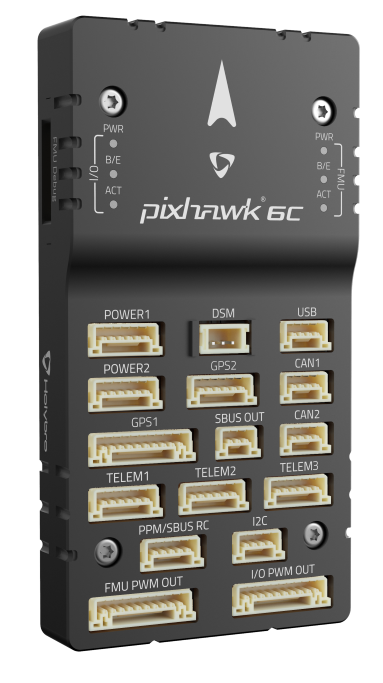
\includegraphics[width=\linewidth]{img/pixhawk6c.png}\\[-1mm]
{\small\textbf{Pixhawk 6C} — автопилот для ArduPilot/PX4}
\end{minipage}\hfill
\begin{minipage}[b]{0.30\linewidth}\centering
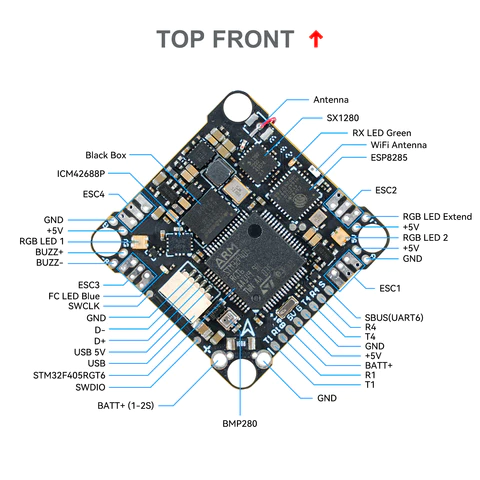
\includegraphics[width=\linewidth]{img/f405-top.png}\\[-1mm]
{\small\textbf{F405 AIO} — FPV-контроллер для Betaflight/INAV}
\end{minipage}\hfill
\begin{minipage}[b]{0.35\linewidth}\centering
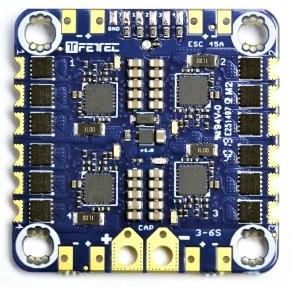
\includegraphics[width=\linewidth]{img/esc4in1.jpg}\\[-1mm]
{\small\textbf{ESC 4-в-1} — четыре регулятора на одной плате}
\end{minipage}
\caption{Полётные контроллеры и регулятор оборотов {\color{gray}\scriptsize(фото: ArduPilot Wiki)}}
\end{figure}

\photo{0.85\linewidth}{f405-wiring.png}{Типовая схема подключения FPV-контроллера: камера, цифровой VTX, приёмник ELRS/TBS, GPS, пищалка, светодиоды}{ArduPilot Wiki}

\subsection{Регуляторы оборотов (ESC)}
\term{ESC} (Electronic Speed Controller) превращает постоянное напряжение батареи в трёхфазное для бесколлекторного мотора, переключая MOSFET-ключи. Характеристики: \textbf{ток} (например, 45\,А длительно), \textbf{напряжение} (3–6S), прошивка (\textbf{BLHeli\_S}, \textbf{Bluejay}, \textbf{BLHeli\_32}, \textbf{AM32}) и протокол связи с ПК (PWM, OneShot, MultiShot, \textbf{DShot} — см. раздел 6). \term{Двунаправленный DShot} передаёт обороты мотора обратно в ПК для RPM-фильтра.

\subsection{Моторы}
\begin{table}[H]\centering\small
\renewcommand{\arraystretch}{1.3}
\begin{tabularx}{\linewidth}{@{}p{34mm} X@{}}
\toprule
\textbf{Коллекторные} (brushed, 6×15, 8×20~мм) & Щётки + коллектор. Дёшевы, управляются одним транзистором (ШИМ). Износ щёток, малый ресурс. Только микро-дроны и игрушки. \\
\textbf{Бесколлекторные} (BLDC, brushless) & Нет щёток, коммутацию делает ESC. Высокий КПД и ресурс, большая мощность. Стандарт для всех дронов. \\
\quad — \textbf{outrunner} & Вращается внешний колокол с магнитами, статор с обмотками неподвижен внутри. Большой момент — прямой привод пропеллера. Используется на дронах. \\
\quad — \textbf{inrunner} & Вращается внутренний ротор. Высокие обороты, малый момент — для импеллеров, машинок, с редуктором. \\
\bottomrule
\end{tabularx}
\caption{Виды моторов}
\end{table}

\begin{figure}[H]\centering
\begin{minipage}[c]{0.3\linewidth}\centering
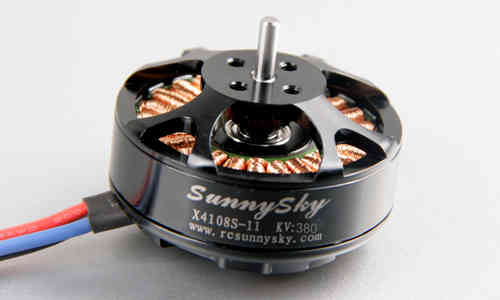
\includegraphics[width=\linewidth]{img/motor-sunny.jpg}\\
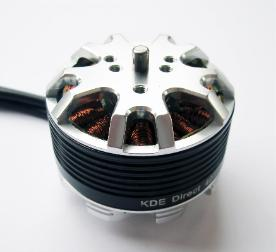
\includegraphics[width=0.8\linewidth]{img/motor-kde.jpg}\\
{\scriptsize\color{gray}(фото: ArduPilot Wiki)}
\end{minipage}\hfill
\begin{minipage}[c]{0.66\linewidth}
\begin{keybox}[Как читать маркировку мотора: \texttt{2207 1950KV}]
\begin{itemize}[leftmargin=4mm]
\item \textbf{22} — диаметр статора, мм; \textbf{07} — высота статора, мм. Больше статор — больше момент и масса.
\item \textbf{KV} — число оборотов в минуту на 1 вольт без нагрузки.\\
$n \approx KV \cdot U$: $1950 \cdot 16{,}8~\text{В} \approx 32\,760$~об/мин.
\item \textbf{Высокий KV} — маленькие лёгкие пропеллеры, низкое напряжение (гонки, 4S).\\
\textbf{Низкий KV} — большие пропеллеры, высокое напряжение (6S, дальнолёты, грузовые).
\item Типично: 5" на 6S — 1700–1950KV; 7" на 6S — 1300KV; 15" на 6–12S — 100–400KV.
\end{itemize}
\end{keybox}
\end{minipage}
\caption{Бесколлекторные моторы-outrunner}
\end{figure}

\subsection{Пропеллеры}
\begin{itemize}
\item \term{Маркировка}: диаметр × шаг (в дюймах) × число лопастей. \code{5146} или \code{5.1x4.6x3} — диаметр 5,1", шаг 4,6", 3 лопасти. \textbf{Шаг} — расстояние, на которое винт «ввинтился» бы в воздух за один оборот.
\item \term{Больше диаметр} — выше КПД и тяга, но медленнее отклик. \term{Больше шаг} — выше скорость, но больший ток. \term{Больше лопастей} — больше тяги при том же диаметре, но ниже КПД.
\item \term{Направление}: CW (по часовой) и CCW (против часовой). Соседние моторы вращаются в разные стороны, чтобы компенсировать реактивный момент (благодаря этому возможен поворот по рыскания). «Props in» / «props out» — направление вращения относительно рамы.
\item \term{Материалы}: пластик (PC), нейлон со стекловолокном — для FPV (гнутся, не ломают моторы); \term{карбон} — жёсткие, эффективные, для больших коптеров; \term{складные} — для самолётов и мультикоптеров, которые переносят в рюкзаке.
\item \term{Крепление}: на вал с гайкой (M5), T-mount (болты), для микро — на вал с натягом.
\end{itemize}

\begin{figure}[H]\centering
\begin{minipage}[b]{0.32\linewidth}\centering
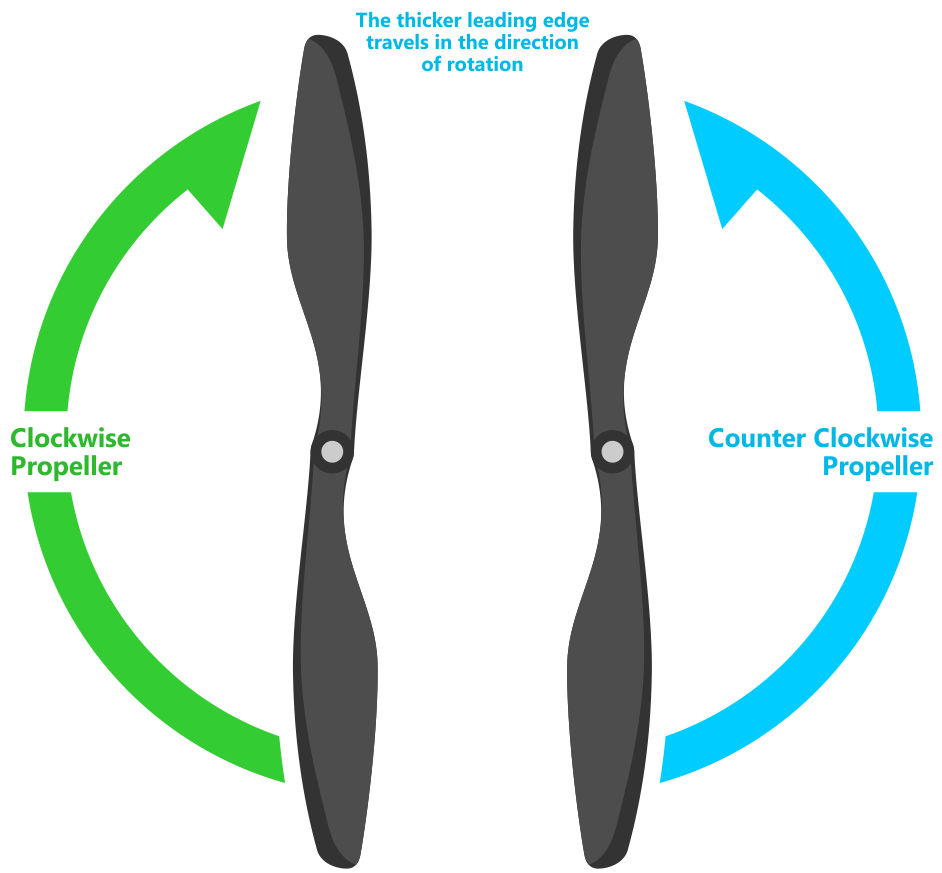
\includegraphics[width=\linewidth]{img/prop-dir.png}\\
{\small Направление вращения CW/CCW}
\end{minipage}\hfill
\begin{minipage}[b]{0.32\linewidth}\centering
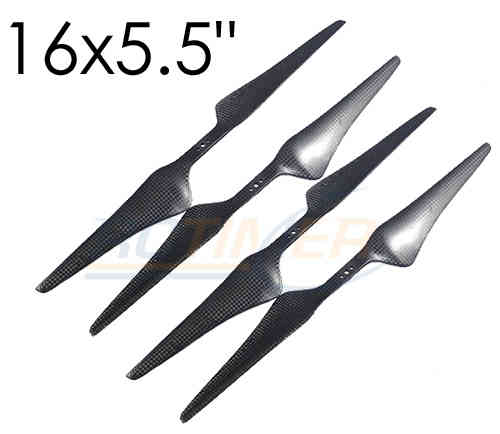
\includegraphics[width=\linewidth]{img/props.jpg}\\
{\small Пластиковые пропеллеры}
\end{minipage}\hfill
\begin{minipage}[b]{0.32\linewidth}\centering
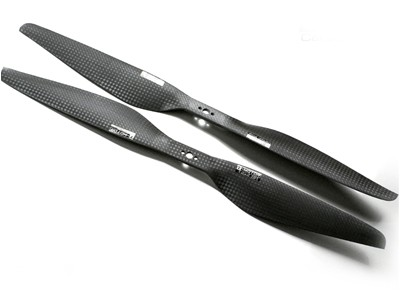
\includegraphics[width=\linewidth]{img/tmotor-props.jpg}\\
{\small Карбоновые пропеллеры для тяжёлых коптеров}
\end{minipage}
\caption{Виды пропеллеров {\color{gray}\scriptsize(фото: ArduPilot Wiki)}}
\end{figure}

\subsection{Типы рам}
\term{Рама} — несущая конструкция, к которой крепится вся электроника. Материал — \textbf{карбон} (углепластик: лёгкий и прочный), реже пластик (whoop), алюминий, стеклотекстолит. Размер задаётся \term{диагональю} (wheelbase) — расстоянием между осями противоположных моторов: 5" $\approx$ \SIrange{210}{230}{\milli\metre}, 7" $\approx$ \SI{300}{\milli\metre}.

\begin{figure}[H]\centering
\foreach \f/\n in {quadx/Quad X,quadplus/Quad +,quadh/Quad H,tri/Трикоптер}{%
\begin{minipage}[b]{0.22\linewidth}\centering
\includegraphics[height=32mm]{img/\f.png}
\end{minipage}\hfill}
\\[3mm]
\foreach \f/\n in {hexax/Hexa X,y6/Y6,octox/Octo X,x8/X8}{%
\begin{minipage}[b]{0.22\linewidth}\centering
\includegraphics[height=32mm]{img/\f.png}
\end{minipage}\hfill}
\caption{Схемы рам и порядок моторов (номер — порядок выхода ПК, CW/CCW — направление вращения). Y6 и X8 — \emph{коаксиальные}: два мотора на одном луче, один над другим {\color{gray}\scriptsize(рисунки: ArduPilot Wiki)}}
\end{figure}

\begin{table}[H]\centering\small
\renewcommand{\arraystretch}{1.25}
\begin{tabularx}{\linewidth}{@{}p{38mm} X@{}}
\toprule
\textbf{Рама} & \textbf{Особенности} \\
\midrule
\textbf{True X} & Моторы на одинаковом расстоянии по всем осям — одинаковое поведение по крену и тангажу. Фристайл. \\
\textbf{Stretched X, Squashed X} & Растянута вдоль / поперёк — оптимизация под гонки или стабильность. \\
\textbf{Deadcat} & Передние лучи разведены, чтобы пропеллеры не попадали в кадр камеры. \\
\textbf{H} & Лучи крепятся к длинной центральной балке — много места для электроники. \\
\textbf{Plus (+)} & Один мотор впереди. Сегодня используется редко. \\
\textbf{Tri} & 3 мотора + сервопривод на хвосте для управления рысканием. \\
\textbf{Hexa, Octo} & 6 и 8 моторов — грузоподъёмность и \textbf{резервирование}: при отказе одного мотора можно сесть. \\
\textbf{Коаксиальные (Y6, X8)} & Компактнее при той же тяге, но нижний винт работает в потоке верхнего (потеря КПД \SIrange{15}{25}{\percent}). \\
\bottomrule
\end{tabularx}
\caption{Особенности рам}
\end{table}

\subsection{Аккумуляторы}
\begin{itemize}
\item \term{LiPo} — литий-полимер. Ячейка: \SI{3.7}{\volt} номинал, \SI{4.2}{\volt} полный заряд, не разряжать ниже \SIrange{3.3}{3.5}{\volt}. \textbf{\emph{n}S} — число последовательных ячеек: 4S = \SI{14.8}{\volt}, 6S = \SI{22.2}{\volt}. \textbf{\emph{m}P} — параллельные.
\item \term{C-рейтинг} — допустимый ток разряда: $I_\text{max} = C \cdot Q$. Пример: \SI{1300}{\milli\ampere\hour}, 100C $\Rightarrow$ \SI{130}{\ampere}.
\item \term{LiHV} — до \SI{4.35}{\volt}/ячейка; \term{Li-Ion} (18650, 21700) — больше ёмкость на массу, меньше ток: для дальнолётов и самолётов.
\item Хранение — при \SI{3.8}{\volt}/ячейка, заряд — балансирным зарядным устройством, в негорючем мешке.
\end{itemize}

\subsection{Камеры}
\begin{table}[H]\centering\small
\renewcommand{\arraystretch}{1.25}
\begin{tabularx}{\linewidth}{@{}p{36mm} X@{}}
\toprule
\textbf{FPV-камера аналоговая} & CMOS-матрица, выход — композитный видеосигнал PAL/NTSC, 600–1200 ТВЛ. Минимальная задержка. Размеры корпуса: nano 14~мм, micro 19~мм, mini 22~мм, full 28~мм. Параметры: фокусное расстояние (1,8–2,1~мм — широкий угол), WDR, чувствительность в люксах. Примеры: RunCam Phoenix, Caddx Ratel, Foxeer Razer. \\
\textbf{FPV-камера цифровая} & Идёт в паре со своим цифровым передатчиком: DJI O3/O4, Walksnail Avatar, HDZero, OpenIPC. 720p–4K. \\
\textbf{Экшн-камера / «голая» GoPro} & Запись качественного видео (4K, стабилизация), отдельно от FPV-камеры. \\
\textbf{Камера на подвесе (гимбале)} & Аэрофотосъёмка: 2- или 3-осевой стабилизатор с бесколлекторными моторами. \\
\textbf{Тепловизор} & ИК-диапазон 8–14~мкм: поиск людей, животных, утечек тепла, ночные полёты. \\
\textbf{Ночная / мультиспектральная} & Съёмка при низкой освещённости; мультиспектр — оценка состояния посевов (NDVI). \\
\bottomrule
\end{tabularx}
\caption{Виды камер}
\end{table}

\begin{figure}[H]\centering
\begin{minipage}[b]{0.30\linewidth}\centering
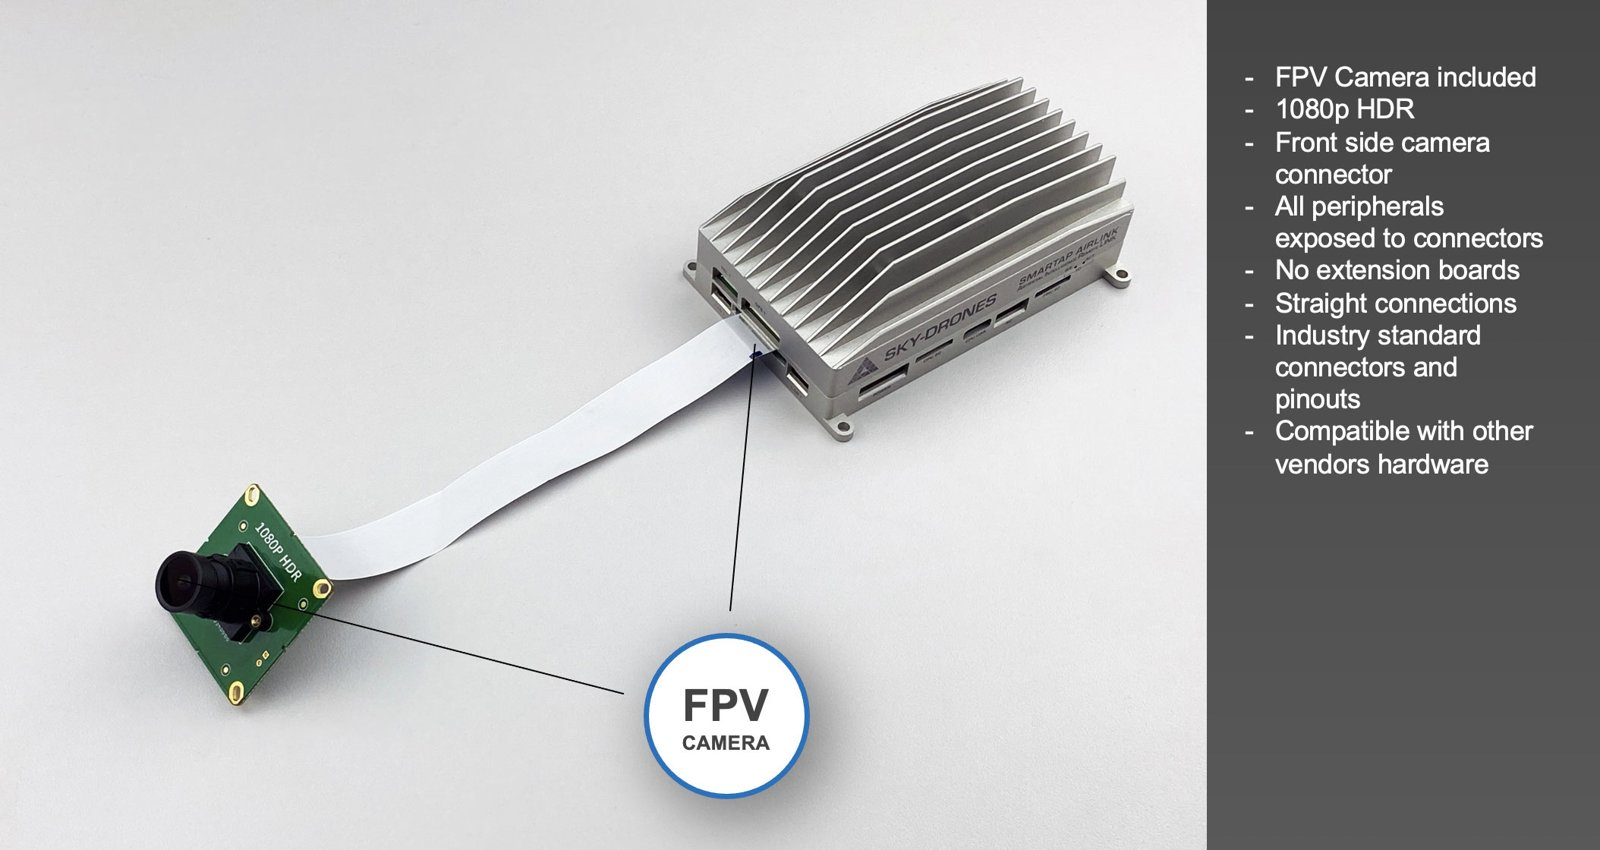
\includegraphics[width=\linewidth]{img/fpvcam.jpg}\\{\small Модуль FPV-камеры}
\end{minipage}\hfill
\begin{minipage}[b]{0.38\linewidth}\centering
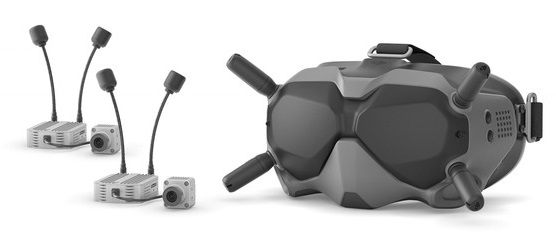
\includegraphics[width=\linewidth]{img/djifpv.jpg}\\{\small Цифровая система DJI: камеры, модули и очки}
\end{minipage}\hfill
\begin{minipage}[b]{0.28\linewidth}\centering
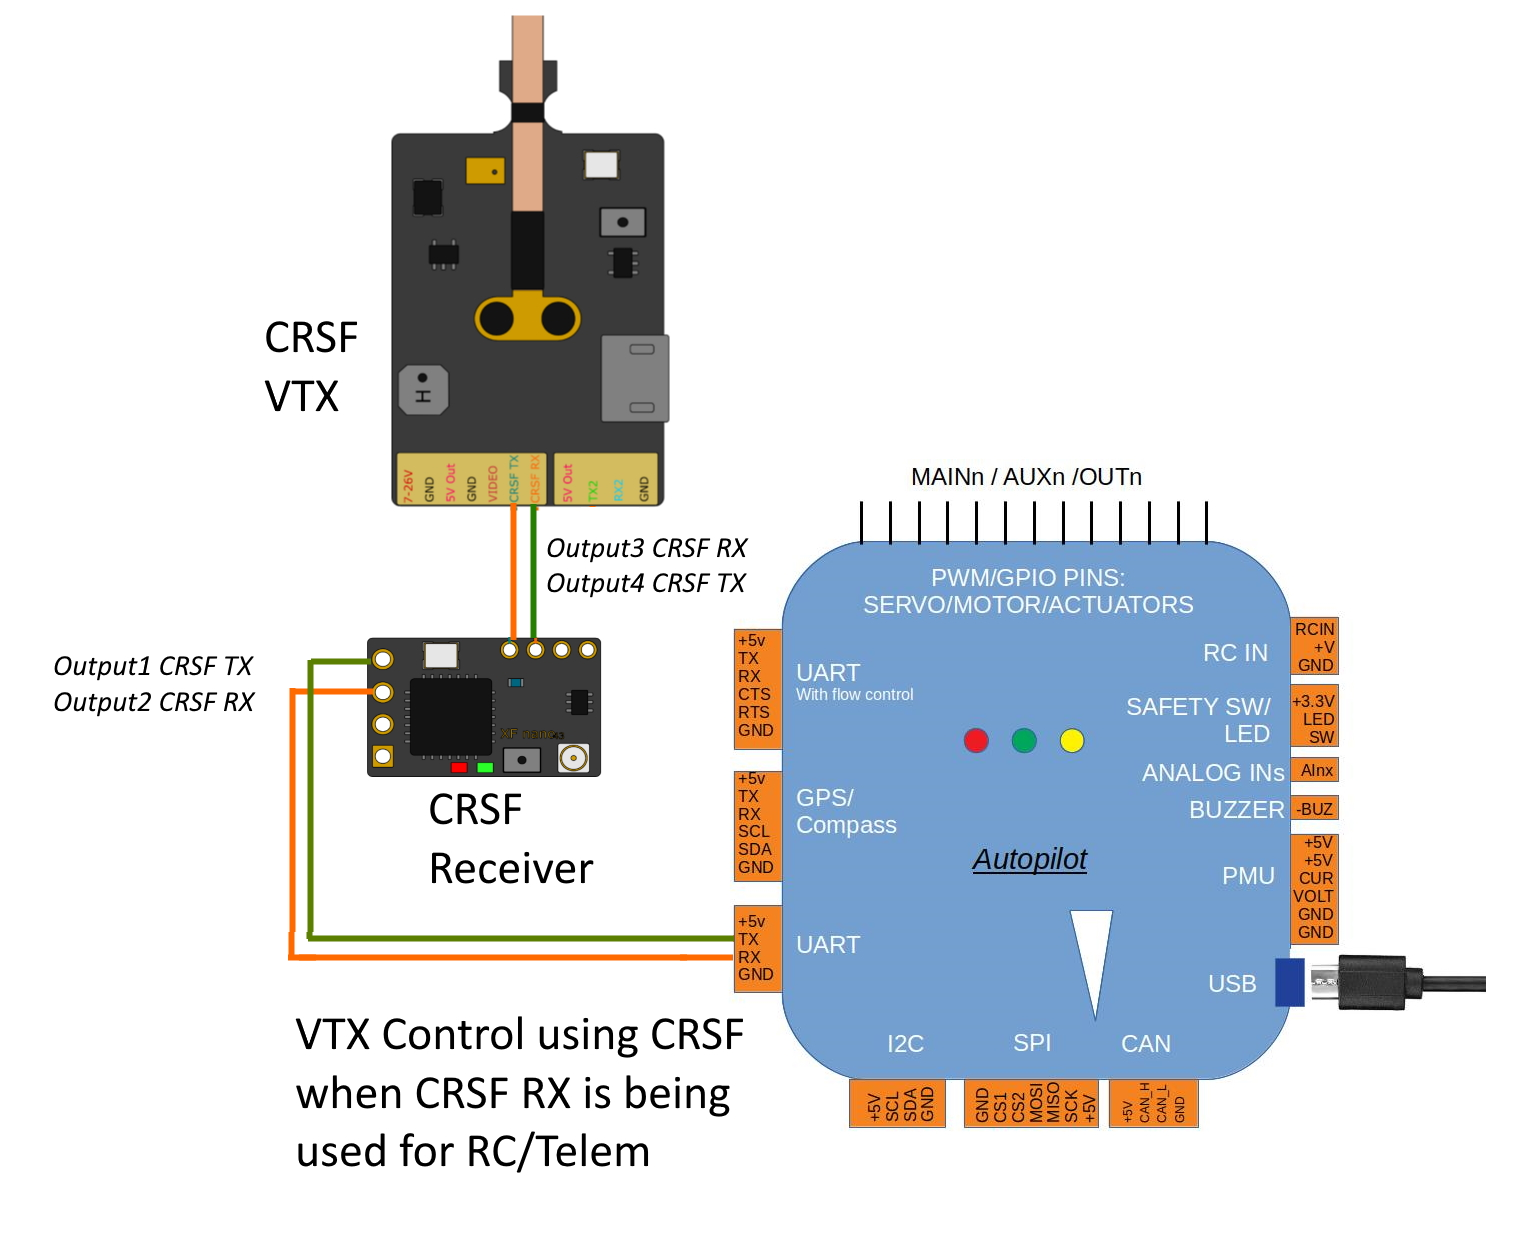
\includegraphics[width=\linewidth]{img/vtx.jpg}\\{\small Подключение VTX с управлением по UART}
\end{minipage}
\caption{Камеры и видеопередатчики {\color{gray}\scriptsize(фото: ArduPilot Wiki)}}
\end{figure}

\subsection{Передатчики и приёмники}
На борту обычно \textbf{три} радиосистемы:
\begin{enumerate}
\item \term{Приёмник управления (RX)} — получает команды от пульта (ELRS, TBS Crossfire, FrSky\ldots). Подключается к ПК по UART (CRSF, SBUS) — см. разделы 6–7.
\item \term{Видеопередатчик (VTX)} — передаёт видео с камеры в очки. Аналоговые: 5,8~ГГц (также 1,2–1,3 и 3,3~ГГц), мощность 25–2000~мВт, 40–48 каналов в диапазонах A, B, E, F (Fatshark), R (Raceband). Управляется от ПК по \textbf{SmartAudio}, \textbf{Tramp} или \textbf{MSP}.
\item \term{Модем телеметрии} — двусторонний канал с наземной станцией (MAVLink): SiK-радио 433/\allowbreak 868/\allowbreak 915~МГц, RFD900, Wi-Fi, LTE-модемы. Часто телеметрия идёт через RC-линк (ELRS, Crossfire).
\end{enumerate}

\subsection{Антенны}
\begin{itemize}
\item \term{Всенаправленные}: \textbf{диполь} (линейная поляризация), \textbf{«клевер»} (cloverleaf), \textbf{«пагода»}, \textbf{Lollipop} — круговая поляризация (RHCP/LHCP). Круговая поляризация уменьшает замирания от отражённого сигнала. \textbf{Поляризация на передатчике и приёмнике должна совпадать!}
\item \term{Направленные}: \textbf{патч}, \textbf{спиральная (helical)}, \textbf{Yagi}, \textbf{moxon} — больше усиление (дальность), но узкий луч, нужно направлять на дрон (часто — трекер).
\item \term{Разъёмы}: SMA, RP-SMA, MMCX, u.FL (IPEX). \textbf{Никогда не включайте передатчик без антенны} — выгорит выходной усилитель.
\end{itemize}

\begin{figure}[H]\centering
\begin{minipage}[b]{0.3\linewidth}\centering
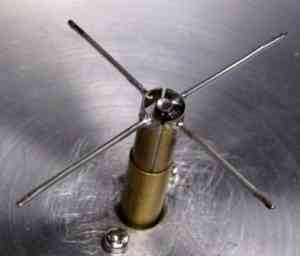
\includegraphics[width=\linewidth]{img/crossantenna.jpg}\\{\small Всенаправленная антенна с круговой поляризацией}
\end{minipage}\hspace{1cm}
\begin{minipage}[b]{0.3\linewidth}\centering
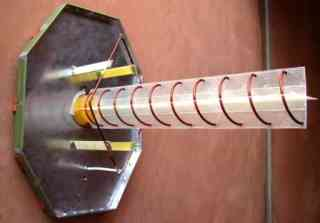
\includegraphics[width=\linewidth]{img/helical.jpg}\\{\small Направленная спиральная (helical) антенна}
\end{minipage}
\caption{Антенны {\color{gray}\scriptsize(фото: ArduPilot Wiki)}}
\end{figure}

\subsection{Прочие компоненты}
\term{GPS/ГЛОНАСС-модуль} с компасом (M8N, M10, BN-880) — позиционирование, возврат домой. \term{PDB / BEC} — распределение питания и стабилизированные 5/9/12~В. \term{Датчик тока} — расход ёмкости. \term{Дальномер, оптический поток} — удержание позиции без GPS. \term{Пищалка} (buzzer) — поиск упавшего дрона. \term{Светодиоды}, \term{парашют}, \term{сбросник} груза.

\begin{exam}
\begin{enumerate}
\item Какие датчики есть на полётном контроллере и зачем каждый?
\item Расшифруйте маркировку мотора 2306 2450KV и пропеллера 5143.
\item Зачем соседние моторы вращаются в разные стороны?
\item Чем отличаются рамы True X, Deadcat и H? В чём плюс гексакоптера перед квадрокоптером?
\item Какой ток может отдать АКБ 6S 1500~мА·ч 120C? Какое у неё напряжение при полном заряде?
\end{enumerate}
\end{exam}
